\appendices

% \section{Ethics and Disclosure}
% \label{sec:disclosure}
% When sending spoofed email messages in our experiments,
% I took deliberate steps to avoid impacting any real users.
% First, I only sent spoofed email messages to accounts that I created ourselves.
% Second, I initially tested each attack by spoofing domains that I created and controlled for this research.
% Once I established that our attacks could succeed using these test domains,
% I ran a small set of experiments that spoofed email from real domains (this was to validate the absence of any unforeseen protection);
% however, these email messages were only sent to our test accounts and did not spoof existing, legitimate email addresses from these domains.
% Finally, all of our email messages contained innocuous text (e.g., ``test'') that would not themselves cause harm.
% % even if a message had somehow been misdelivered,
% % all of our messages contained innocuous content and thus was unlikely
% % to cause harm.

% I have disclosed all of the vulnerabilities and attacks to the
% affected providers. I have received affirmative feedback from
% all affected providers: Zoho not only patched the issue with their ARC
% implementation (also confirmed by Wang et al.~\cite{wang2022revisiting}, who conducted their measurements after the patch) and awarded us a bug bounty, but also is further enhancing its security; Microsoft
% confirmed the vulnerabilities (with severity ``Important'', the highest severity assigned to email spoofing bugs) and awarded us a bug bounty; Gaggle
% confirmed the issues I flagged and stated that they would start
% enforcing DMARC; Gmail has triaged our report and is working on a fix.
% %For the other providers, I have reached out multiple times and are waiting on replies.
% I will report on the full set of disclosure feedback and outcomes in the final version of this paper.


% \section{Measurement Details}
% \label{sec:appendix_measurement_setup}
% This section describes the details of our methodology when performing
% forwarding experiments in
% Sections~\ref{sec:measure_forwarding_mechs_and_arc}
% and~\ref{sec:vulnerabilities_in_the_wild}.
% %
% I start with a set of three new domains under our control.  We
% configure all three with the same SPF configuration, while each of the
% individual domains have a DMARC policy none, quarantine, and reject,
% respectively.  I use these domains in the FROM headers in all of our
% email messages, so that our measurements do not affect users of any
% other domains.

% I then ``warm up'' our domains so that they are treated like any
% other domains by the providers.  I send legitimate email messages
% from these domains that pass SPF, DKIM and DMARC to accounts under our
% control at each email provider.  I also manually mark our email
% messages as ``not spam'' if they are delivered to the spam folder in
% the warm-up stage.  After the warm-up stage, legitimate email messages
% from our domains are properly delivered to account inboxes for all
% email providers.

% I then send legitimate and spoofed email messages from our domains to
% forwarding accounts and record whether a message is forwarded by
% default.  I consider all six providers and four mailing lists as
% forwarders.  I send spoofed email messages from a server I own that
% is not allowed in the SPF records of our domains.

% I study each receiver's behavior for both legitimate and spoofed
% forwarded email messages. I only consider the six mail providers as
% receivers, as mailing lists are rarely the destination of email. We
% configure all forwarders to forward email messages to all receivers
% and record whether each message is delivered to the inbox, spam
% folder, or rejected without delivery by each receiver. I also note
% whether any UI warning indicator is displayed in the native web-based
% MUA.

% I force the forwarding of a spoofed email by manually whitelisting it
% at the forwarder. Whitelisting spoofed email messages could be done at
% most forwarders with a few exceptions. I are not able to whitelist
% spoofed email messages at Yahoo in cases where the spoofed FROM domain
% has DMARC policies quarantine or reject. Additionally, I cannot
% whitelist spoofed email messages at Google and Zoho in cases where the
% spoofed FROM domain has DMARC policy reject.

% I ensure that our measurement results are reliable by repeating the
% above process with another set of three domains and fresh email
% accounts. I are also aware that all mail providers I study have
% implemented anti-spam systems, which could interfere with our
% measurement results. To minimize the interference from those systems,
% I only send email messages with legitimate content. In cases where we
% observe an inconsistency in a provider's behavior between multiple
% trials (potentially due to triggering the anti-spam system), we
% perform additional measurements with fresh accounts.


%The appendices below present screenshots of successful attacks, discuss our ARC measurements in more detail, and describe additional details for the attacks in Sections~\ref{subsec:attack_relaxed_forwarding_validation},~\ref{subsec:attack_zoho_arc}, and~\ref{subsec:attack_none_mailing_list}.
\newpage
\section{ARC Adoption in the Wild}
\label{sec:arc_adoption_and_trust}
\begin{table}[t]
  \centering
\begin{tabular}{l|llll}
  \toprule
  & \multicolumn{3}{c}{\textbf{Added by}} \\
\textbf{Received by} & Gmail & Zoho & Fastmail & Pobox\\
\midrule
Gmail    & \checkmark     &                &       \checkmark  & \checkmark\\
Outlook  & \checkmark     &               &         & \\
Zoho     & \checkmark     &     & \checkmark      & \checkmark    \\
Fastmail & \checkmark     & \checkmark    & \checkmark   & \checkmark\\
Pobox    & \checkmark     &               & \checkmark   & \checkmark\\
\bottomrule
\end{tabular}
\caption{Trust of ARC headers between providers.\label{tab:trust_of_arc_between_providers}}
\end{table}

\label{sec:appendix_arc_measurement}
Five email providers (Gmail, Outlook, Zoho, Fastmail, and Pobox) and two mailing list services (Google Groups and Mailman) implement ARC validation.
% I note that when forwarding, Outlook only adds ARC headers to email messages originated from itself.
% \grant{Is this last sentence important or referenced later on? If not, I can probably remove it, or move this detail to that later section.}
Because ARC is still an experimental protocol, many email providers only evaluate ARC headers added by a small set of other providers whom they trust~\cite{Senderau57:online}.
Based on measurements through test accounts that I created, Table~\ref{tab:trust_of_arc_between_providers} shows the ARC trust relationships among the providers I tested:
Gmail trusts ARC headers added by Fastmail, Pobox and itself; Outlook trusts ARC headers added by Gmail; Zoho trusts ARC headers added by Gmail, Fastmail, Pobox and itself;  Fastmail trusts ARC headers added by Gmail, Zoho, Pobox and itself; and Pobox trusts ARC headers added by Gmail, Fastmail and itself.

We also note two details.
First, I cannot test whether other providers trust ARC headers added by Outlook. ARC headers are only evaluated when a forwarded email fails DMARC authentication checks.
However, in our experiments, Outlook only adds ARC headers to certain email messages that will pass DMARC authentication checks after forwarding.
This design prevents us from testing which providers trust Outlook's ARC headers.
% Thus, I cannot determine if other providers evaluate and trust ARC headers added by Outlook. % are evaluated and trusted by other providers.
Second, our results suggest that Zoho does not add ARC headers when forwarding messages internally between Zoho accounts, so I leave that cell empty in the table.

\section{Additional Implementation Errors}
\label{sec:implementation_errors_additional}
We detail two other implementation errors identified during our measurement. These two errors play minor roles in the attacks I discover.
\subsection{Ignoring Security Protocols}
\label{subsec:no_dmarc}
Systems that assume every email is legitimate tend not to enforce DMARC. Instead, they will permissively accept
email messages, even if they fail DMARC authentication checks and the
purported FROM domains have a stricter DMARC policy of \textsc{Quarantine} or
\textsc{Reject}. Such assumptions can create serious security issues.

From our experiments, I found
one mailing list provider (Gaggle) and three mail providers (Freemail, Mail2World and Runbox) that do not enforce
DMARC.
Beyond delivering spoofed email to users and allowing spoofed email to be forwarded, we
show later (Section~\ref{subsec:attack_none_mailing_list}) that
incorrect enforcement, combined with the standard forwarding
modifications that Gaggle applies to email headers, allows an attacker
to abuse Gaggle. Spoofed email messages that initially fail
DMARC authentication will receive a fresh set of headers that
correctly pass SPF and DMARC validation after they are forwarded
through a Gaggle-operated mailing list.

\begin{figure}[t]
  \centering
%% \centerline{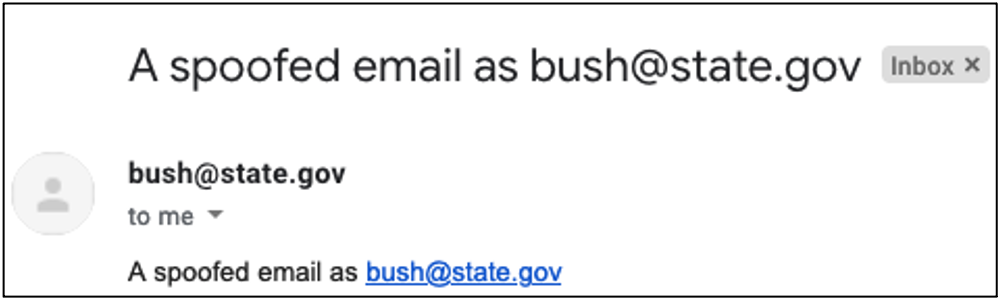
\includegraphics[width=\columnwidth]{graphs/ss_outlook_open_forwarding.png}}
{
    \setlength{\fboxsep}{0pt}
    \setlength{\fboxrule}{0.5pt}
    \fbox{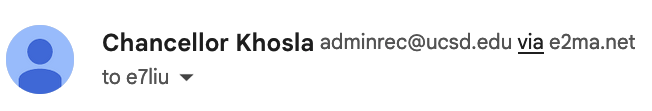
\includegraphics[width=\columnwidth]{graphs/ss_gmail_via_ui.png}}
}
%  \vspace*{-0.2in}
  \caption{Gmail annotating the sending address of an email. 
}
%\vspace*{-0.1in}
\label{fig:gmail_via}
\end{figure}

\subsection{Gmail UI Bug}
\label{subsec:ui_bug}
After a receiver accepts and processes email,
the user's mail user agent (MUA) displays the message for viewing.
Thus, MUAs and their UI warnings serve as the last line of defense against spoofed email messages.
However, previous work~\cite{hu_end--end_nodate,shen2020weak,chen2020composition} has found multiple security issues in various MUAs, especially on mobile platforms.
In our experiments, I focus on the native MUAs (web interfaces) provided by the nine email platforms in our study.
These MUAs not only have widespread usage, as the default MUA for many users,
but are also maintained by the email providers and tend to have better security practices.
% I focus on native MUAs because they tend to do their due diligence on the implementing a comprehensive UI warning system.

Among all native MUAs, only Gmail, Onet and Zoho have implemented warning
systems that display UI indicators when an email is forwarded or fails
DMARC authentication.  Gmail, for instance, annotates the
sending address (e.g., \dns{adminrec@univ.edu} \textit{via} \dns{e2ma.net} as shown in Figure~\ref{fig:gmail_via}).

%% Figure~\ref{fig:gmail_ui_normal} shows an example of Gmail displaying
%% a UI notice for a forwarded message (in this case via
%% \dns{gmail.com}).

However, I observed a bug in Gmail's warning system for a subset of forwarded
messages. In particular, Gmail does not display an indicator for a forwarded
email message if (1) it does not contain any DKIM headers, and (2) it has the
same domain in both the \textsc{MAIL FROM} and \textsc{FROM} headers.
%Figure~\ref{fig:gmail_ui_bug} shows an example of such an email message.
This policy does not pose a problem in single-sender email settings, because adversaries still need to bypass SPF and DMARC.
However, I present a new attack that uses this bug in conjunction with forwarding and other vulnerabilities to deliver spoofed email messages that look no
different than legitimate messages (Section~\ref{subsec:attack_relaxed_forwarding_validation}).
% \geoff{where in \ref{subsec:attack_relaxed_forwarding_validation}?}\alex{updated \ref{subsec:attack_relaxed_forwarding_validation}}
% \section{Mitigation}
% The attacks I demonstrate highlight the complicated interactions between email forwarding and existing anti-spoofing mechanisms.
% Below I propose several defenses that email platforms can use to mitigate each attack.
% While these defenses use existing and practical mechanisms, they often require changes by multiple or unaffected parties across the email ecosystem (e.g., changes by forwarding providers to protect downstream recipients).
% This quagmire underscores the complexity that email forwarding adds to anti-spoofing measures and illustrates the need for more holistic and comprehensive approaches to improving email security.

% To mitigate the first three attacks I demonstrate in this paper, I recommend all mail service providers disable \emph{open forwarding}, and instead require confirmation by the forwarding recipient as part of the process.
% Although this design will incur additional effort by every user who sets up forwarding, it will mitigate these three attacks, since all of them leverage the \emph{open forwarding} feature of email platforms.
% Additionally, I suggest that providers enforce rejection (outright dropping) of email messages that fall under the scope of a DMARC reject policy. Had Outlook rejected the spoofed email messages in the first place, the impact of the first attack (Section~\ref{subsec:attack_open_forwarding}) would narrow substantially.
% Unfortunately, both of these defenses reflect a case of misaligned
% %harms
% incentives: the recipients of spoofed email (\eg, spam and phishing) cannot implement this change,
% but instead need to rely on the entire ecosystem of providers and forwarding services to adopt such defenses.

% Email providers can mitigate the second attack (\S~\ref{subsec:attack_relaxed_forwarding_validation}) by eliminating the relaxed validation policies.
% This approach would protect their users from receiving spoofed email without relying on changes by other platforms or services.
% However, to ensure that benign forwarding does not break, providers will likely need to implement ARC validation, which requires forwarders from external services to implement it and potentially introduces new problems such as trust issues.
%  % Finally, while relaxed validation certainly helps increase the deliverability of forwarded email messages, I recommend implementing ARC and stick with DMARC policy when possible.

% For the final attack that abuses mailing lists, I suggest two different defenses that trade usability for security.
% % As for the attack on mailing lists, there exists two types of defense mechanisms that trade usability for security.
% First, list owners can turn on message moderation or set their mailing lists to be private.
% These measures increase the difficulty of performing email spoofing attacks,
% but do not rule out the attack entirely. A dedicated attacker might
% nonetheless identify a member of the mailing list and craft an email
% that fools a list's moderator.
% Second, some mailing list services, such as Listserv, support confirm-before-send~\cite{OnmyLIST7:online}, which requests confirmation from the (true) sender address before delivery.
% However, the additional overhead this imposes for each message might prevent widespread use.
% As a compromise, I recommend that mailing lists turn on this option by
% default for any incoming email that fails DMARC authentication checks.

% % While these short-term fixes will significantly reduce the exposure to the
% % attacks I have described here, I believe ultimately email requires a more
% % solid security footing if it is to effectively resist spoofing attacks going forwards.


\section{Additional Attack Screenshots}
% \paragraph{Additional Screenshots}
We ran a small set of experiments that spoofed email impersonating real domains to validate the attacks described in Section~\ref{sec:attacks}.
Our experiments confirmed that these attacks succeed.
Below, I present the screenshots of spoofed email messages successfully delivered to users' inboxes.

For the attack described in Section~\ref{subsec:attack_relaxed_forwarding_validation}, Figure~\ref{fig:ss_gmail_via_outlook} shows a spoofed message forwarded via a personal Outlook account to a Gmail account I created, and delivered to the recipient's inbox without any security warnings.
The spoofed address in this example impersonates a sender at \dns{alipay.com} (a prominent Chinese payment company with a DMARC policy of \textsc{Quarantine}).

For the attack described in Section~\ref{subsec:attack_zoho_arc}, Figure~\ref{fig:ss_zoho_arc} illustrates that this attack succeeds
without any security warnings, even though the spoofed domain in our
experiment, \dns{facebook.com}, has a DMARC policy of \textsc{Reject}.


% \paragraph{Additional Details for the Attack in Section~\ref{subsec:attack_relaxed_forwarding_validation}}
\section{Additional Details for the Attack in Section~\ref{subsec:attack_relaxed_forwarding_validation}}
\label{sec:append_change_behavior_details}
This section makes three additional observations about the attacks on
providers with relaxed forwarding validation as described in
Section~\ref{subsec:attack_relaxed_forwarding_validation}.

First, in addition to forwarding from personal Outlook accounts, an
adversary can also forward from personal accounts with other providers
(\eg, Fastmail) to Gmail recipients.
As mentioned earlier in Section~\ref{subsubsec:relaxed_validation}, there is an additional caveat: the \textsc{TO} header of the spoofed email cannot be the same as victim's email address.
An astute recipient might see that the \textsc{TO} field corresponds to someone else's email account, and become suspicious about the email's validity.
To reduce suspicion in this case, the adversary can set the
human-readable name portion of the email's \textsc{TO} header to
``me'' or the victim's name (while keeping the address different).

Second, adversaries need to leverage popular mail providers as forwarders in this attack; they cannot exploit relaxed forwarding validation by using their own servers as forwarders.
In our experiments, I tested using both a personal Outlook account as well as a mail server I controlled as forwarders.
The first version results in successful attacks delivered to user inboxes, but the latter did not.
We suspect this outcome is because our mail server domain has lower reputation than Outlook's mail servers.

Finally, in Section~\ref{subsec:attack_relaxed_forwarding_validation}, I demonstrate the attack against a recipient using Gmail. A similar attack can be mounted against Outlook recipients by
forwarding via a personal Fastmail account. This attack allows an
adversary to spoof email messages from many domains that have a DMARC
policy \textsc{None} to arbitrary Outlook recipients.\footnote{Similar to the caveats described in
Section~\ref{subsubsec:quarantine_instead_of_reject}, I observe that Outlook applies
additional restrictions to a small set of high-profile domains with a
DMARC policy of \textsc{None} (e.g., \dns{citizensbank.com}), which blocks the delivery of spoofed emails from these domains.}
Figure~\ref{fig:attack_none_ms} shows a spoofed email message
forwarded via a personal account to an Outlook account I created, and
delivered without any security warnings. The spoofed FROM header in
this example impersonates a sender at \dns{lesechos.fr} (a French
financial newspaper with a DMARC policy of \textsc{None}).

\begin{figure}[t]
  \centerline{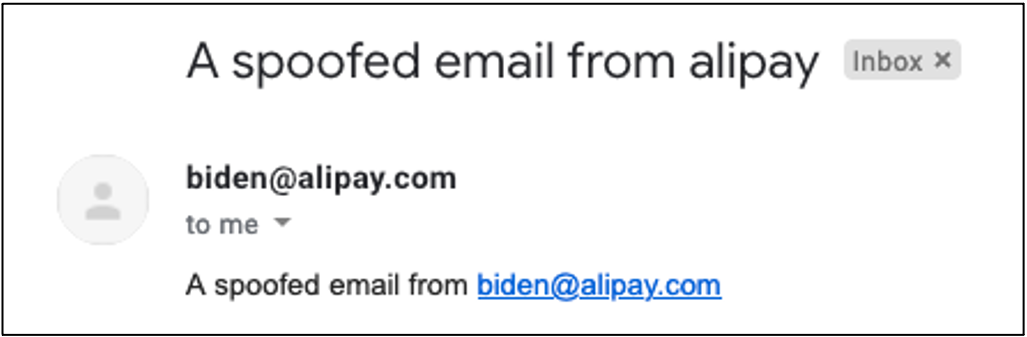
\includegraphics[width=\columnwidth]{graphs/ss_gmail_via_outlook.png}}
  \centering
  \caption{Email spoofing \dns{biden@alipay.com} via Outlook.}
  \label{fig:ss_gmail_via_outlook}
  \end{figure}


\begin{figure}[t]
  \centerline{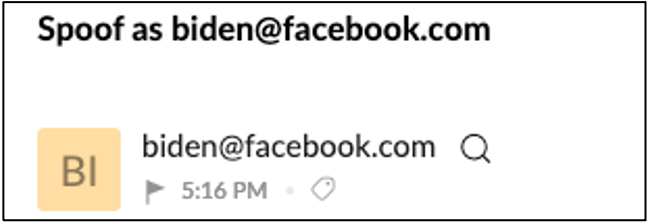
\includegraphics[width=\columnwidth]{graphs/ss_zoho_arc.png}}
  \centering
  \caption{Email spoofing \dns{biden@facebook.com} via Fastmail.}
  \label{fig:ss_zoho_arc}
  \end{figure}

\begin{figure}[t]
\centerline{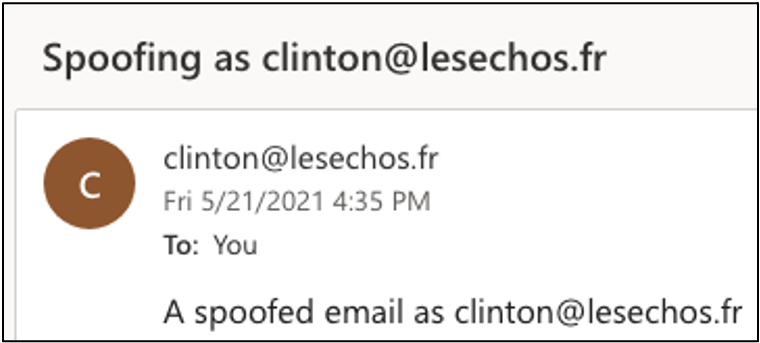
\includegraphics[width=\columnwidth]{graphs/ss_outlook_none.png}}
\centering
\caption{Spoofed email message taking advantage of Outlook's relaxed forwarding validation policy.}
% \geoff{let's see if Stefan notices this screenshot}}
\label{fig:attack_none_ms}
\end{figure}


\section{Additional Details for the Attack in Section~\ref{subsec:attack_zoho_arc}}
\label{sec:appendix_zoho_attack_details}
% \paragraph{Additional Details for the Attack in Section~\ref{subsec:attack_zoho_arc}}
Adversaries can broaden the scope of the attack described in Section~\ref{subsec:attack_zoho_arc} by using a forwarding
account at any email provider that Zoho trusts for ARC purposes,
including Gmail, and routing their spoofed email through multiple forwarding hops.
In particular, an attacker can obtain ARC headers in one forwarding hop via Gmail, and then bypass Gmail's lack of open forwarding by forwarding the email through a second account that does allow open forwarding (\eg, Outlook).
% The attacker can use a Gmail
% account to obtain the necessary ARC headers by including this account as an additional forwarding hop.
% For example, the attacker could create a second
% forwarding account on a platform that has open forwarding (\eg,
% Outlook).
For example, first, the attacker would send their spoofed email message
to their Gmail account, which they configured to forward to their
malicious Outlook account.
During the forwarding process Gmail will
attach a set of ARC headers to the email message.
Next, the spoofed email will arrive at their malicious Outlook account, which then forwards the email to any arbitrary Zoho recipient (because Outlook
supports open forwarding).
This forwarded email message will contain Gmail's attached ARC headers, enabling the attack to successfully pass DMARC validation checks as a result of Zoho's vulnerable ARC implementation.

Using our test accounts, I validated that this multi-hop attack variation
successfully delivers spoofed messages to the inbox of a Zoho recipient
without any warnings.






\section{Additional Details for the Attack in Section~\ref{subsec:attack_none_mailing_list}}
% \paragraph{Additional Details for the Attack in Section~\ref{subsec:attack_none_mailing_list}}
\label{sec:append_mailing_list_details}

% \subsection{Abusing Gaggle.email}

\begin{figure}[t]
\centering
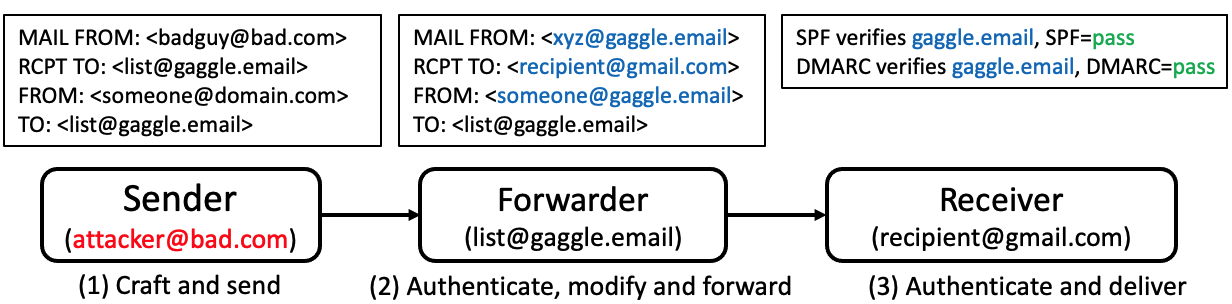
\includegraphics[width=\columnwidth]{graphs/mech_gaggle.png}
\centering
\caption{Attack flow for Gaggle.}
\label{fig:gaggle_email_mech}
\end{figure}

In addition to the attacks described in
Section~\ref{subsec:attack_none_mailing_list}, I found
additional attack variants related to Gaggle.
Figure~\ref{fig:gaggle_email_mech} shows an example of an attack that
abuses Gaggle's use of REM + MOD forwarding
(Section~\ref{sec:measure_forwarding_mechs_and_arc}). This attack works
regardless of the DMARC policy of the spoofed address's domain.  First, an
attacker chooses an address to spoof (\dns{someone@foo.com}) that is
allowed to send to a mailing list on a vulnerable provider
(\dns{list@gaggle.email}), and sends a spoofed email message
purporting to come from that address.  This spoofed email will fail
DMARC validation, but because Gaggle does not enforce DMARC
(Appendix~\ref{subsec:no_dmarc}), it will forward the email to the
mailing list's recipients as normal (Stage 2).  Since Gaggle uses a
REM + MOD forwarding process, it will rewrite the \textsc{MAIL FROM}
header to use the mailing list's domain (\eg, a
new \textsc{MAIL FROM} address of \dns{xyz@gaggle.email}).
%\grant{Similar to earlier, I should be more precise.}
Finally, when the spoofed email message arrives at the recipient's mail server,
it will properly pass SPF validation and DMARC alignment checks:
the rewritten \textsc{MAIL FROM} domain allows the mailing list to send on its behalf, and the domain matches the \textsc{FROM} address's domain (\dns{gaggle.email}).

% \subsection{Other Details}
% Below, I note one additional detail\alex{fix this number} about this attack.

Additionally, I note that mailing list software such as Listserv and
Mailman require a backend MTA.  In our experiments I used Postfix
with DMARC turned on, a configuration which follows good security
practice.  However, in practice many organizations might not use this
configuration because many MTAs (including Postfix) do not enforce
DMARC by default.  In these cases, the attacker can spoof email from any
target domain, regardless of its DMARC policy, much like the attack
against Gaggle.


%\section{Limitations}
%Most of the attacks described in this paper require that the attacker has an account on an email forwarding service and can configure the account to forward email message to the target account. Thus, massively and automatically performing the attacks described in this paper can be challenging. Automating the attacks (e.g., via automated account creation) is out of scope for this work.
